For a real world recognition task, an algorithm that can continuously adaptive to new labels just like the human does, is always very attractive and practical.
In this section, we propose an adaptive method for learning new categories with a few target examples using the feature representations from GoogLeNet. By warm start the parameters of the classifiers, our method can effectively learning new categories. The experiment results show that our method is able to adapt new categories with just a few examples and converges faster compared to method without warm start.
For the rest part of this section, we first discuss the limitation of some previous domain adaptation approaches for our task, then we introduce our method and show the improved performance on the same task.

\subsection{Limits of previous approaches}
From previous studies, there are two kinds of approach to solve our task. The first approach is to fine-tuning the deep CNN with the target examples incorporating with the sources ones.
Fine-tuning the deep CNN model focuses on learning good feature representations from the images and using linear models for classification. From Section \ref{sec:ft}, we successfully use this approach to transfer the knowledge from a general domain to our food domain and achieve an accuracy of 78.11\%. Indeed, deep CNN can learn distinctive features effectively and by taking advantage of this, this approach achieved some impressive results from previous studies\cite{Chatfield14} \cite{zeiler2014visualizing}. However, fine-tuning on deep CNN requires an ample amount of labeled target data and sometimes could degrade the performance when the labeled examples are scarce\cite{hoffman2013one}. There are many hyperparameters that affect the performance of deep CNN and sampling noisy is a major problem that makes fine-tuning deep CNN on limited examples prone to overfitting \cite{srivastava2014dropout}. Apart from these reasons, fine-tuning the whole network requires intensive computational resources which is not an efficient approach for learning new categories.

Rather than learning efficient representations, other approaches are more focused on dealing with the representations learned from conventional feature extraction methods for domain adaptation \cite{yang2007adapting} \cite{aytar2011tabula}. Supervised domain adaptation models, such as Adaptive-SVM (A-SVM) and PMT-SVM, try to utilize the knowledge from source domain and apply to target domain, assuming that the classifier of the new category should have some linear relationship with the classifiers of the source categories. Indeed, they work well when the categories are geometrically similar. However, for deep representation from deep CNN, this assumption doesn't help much.

From empirical experiments, we find that adaptive methods suffer as the difference of source and target categories increases. Table \ref{tab:su_domian} shows some experiment results for two typical domain adaptation methods (A-SVM \& PMT-SVM) and two classifiers without any adaptation in a binary classification scenario. For adaptation methods, we manually choose the similar/identical source categories for the target ones. For the those categories which we fail to find even similar category in source domain, we just choose the category whose representations are most similar to the target one measured by cosine similarity \cite{aytar2011tabula}. The parameters used in these methods are set as their default. From the results of our simple experiment, we can see that using deep representation, even to adapt identical category, the improvement of the adaptation technique is not significant compared to raw models.

For our food recognition task, we expect to find a method that can learn new food with just a few labeled images. From Section \ref{sec:ft}, we show that shallow linear model trained on small dataset can achieve competitive result with deep representation. This indicates that deep representation can adjust the dataset bias and help for adaptation. To adapt new category with deep representation, we propose a Incremental adaptive learning method.
% Table generated by Excel2LaTeX from sheet 'Sheet1'
\begin{table*}[htbp]
  \centering
  \caption{Average Precision for A-SVM, PMT-SVM, SVM and Logistic Regression trained with deep representation. Source categories without * are determined by cosine similarity}
    \begin{tabular}{cccccc}
    \toprule
    Target Category & Source Category & A-SVM  & PMT-SVM & SVM &LR\\
    \midrule
%    Green salad & Caesar salad & 0.1627 & 0.1622 \\
    Doughnut & Doughnut & 0.4771 & 0.4735 &0.4781&0.4554\\
    Caesar salad &  Caesar salad & 0.9488 & 0.9496 &0.9498&0.9486\\
    White rice  & Fried rice & 0.8118 & 0.7932 &0.7932&0.9004\\
    Oatmeal & French onion soup* & 0.0345 & 0.0381 & 0.0347 &0.0454\\
    Pork cutlet & French fries* & 0.0446 & 0.0381 &0.0450& 0.0837\\
    \bottomrule
    \end{tabular}%
  \label{tab:su_domian}%
\end{table*}%

%As far as we know, few study has shown that there is an approach that can solve our task. Therefore, we propose an incremental adaptive learning algorithm to solve this problem.
\subsection{Incremental adaptive learning for new category}
From previous section we can see that linear assumption doesn't help classifier to adapt new category with deep representation significantly.
In Table \ref{tab:weight_sim} we show the weight similarity of the classifiers for different categories and observe that even for similar categories, the parameters of the classifiers are quite different. So we think that if we warm start the classifier of the new category with some parameters that are different from any learned ones for optimization, the classifier can be trained more efficiently. Warm start is to initialize the model with some chosen parameters and has been used in many linear models.
Chu et al. recently proposed a warm start approach for parameter search in linear model and by iteratively updating the parameters optimized from previous knowledge, their algorithm can search the optimal value for a specific task\cite{chuwarm}. Inspired by this, we propose a warm start adaptive learning algorithm that can adapt new categories from the target domain.% in an incremental learning mode.

To choose the parameters that are different from previous learned categories, we introduce a negative classifier which is trained using all examples from the learned categories as negative examples. This negative classifier tends to reject all the learned categories and it should be more effective to start the new classifier with its parameters for optimization. We uses logistic regression to classify the representations obtained from deep CNN because from Table \ref{tab:mini} we can see that logistic regression performs well with a few examples.

To learn multiple new categories, instead of learning the them once, our method adapts one category in each step and updates all the parameters for the learned classifiers as well as the negative one. The algorithm terminates while all the new categories are leaned.
For each step, given $M$ learned categories in set $S$ and a new category $t$ from target domain, there are $M$ binary classifiers $F=\left\{ {{f}\left( {{w_i},{b_i}} \right)} \right\}_{i = 1}^M$ for each learned category. We use $\mathcal{P^-}_i$ and $\mathcal{P^+}_i$ to denote the negative examples and positive examples for the i$th$ class respectively. The negative classifier $\hat{f}(\hat{w},\hat{b})$ is trained with $\mathcal{P^-}_{neg}=S$. The classifier $f_t$ for the new category $t$ is initialized with $\left\{\hat{w},\hat{b}\right\}$ and trained with $\mathcal{P^-}_t\bigcup\mathcal{P^+}_t$ for $\mathcal{P^+}_t=t$ and $\mathcal{P^-}_t=S$. Then we update the negative classifier $\hat{f}$ with negative examples $\mathcal{P^-}_{neg}=S\bigcup t$. We use Stochastic Gradient Descent (SGD) to update the parameters for all the binary classifiers as well as the negative classifier. The complete strategy for our method is given in Algorithm \ref{algo:ws}.
\begin{algorithm}
  \caption{Warm start adaptation with negative classifier}\label{algo:ws}
  \begin{algorithmic}[1]
    \REQUIRE Source domain $S = \{ {s_i}|i = 1,..M\} $, Target domain $T = \{ {t_j}|j = 1,..N\} $, Classifier $F = \{\emptyset\}$
    \ENSURE $F$\\
    \FORALL {$i\in M$}
         \STATE $\mathcal{P^+}_i \leftarrow s_i, \mathcal{P^-}_i\leftarrow \{S-s_i\}$\\
          Train ${{f_i}\left( {{w_i},{b_i}} \right)}$ with $\mathcal{P^+}_i\bigcup\mathcal{P^-}_i$, $F\leftarrow F\bigcup f_i$
    \ENDFOR
    \STATE Training negative $\hat{f}\left( {\hat{w_i},\hat{b_i}} \right)$ with $\mathcal{P^-}_{neg}=S$
    \WHILE {$t_j  \notin S$}
         \FORALL {$i\in M$}
             \STATE $\mathcal{P^+}_i \leftarrow s_i, \mathcal{P^-}_i \leftarrow S-s_i+t_j$ \\
              Update ${{f_i}\left( {{w_i},{b_i}} \right)}$ with $\mathcal{P^+}_i\bigcup\mathcal{P^-}_i$
        \ENDFOR
        \STATE Initialize $f_j$ with $(\hat{w},\hat{b})$
        \STATE $\mathcal{P^+}_j \leftarrow t_j, \mathcal{P^-}_j\leftarrow S$
        \STATE Train $f_j$ with $\mathcal{P^+}_j\bigcup\mathcal{P^-}_j$.
        \STATE $F\leftarrow\ F\bigcup f_j$
        \STATE $S\leftarrow S\bigcup t_j, M\leftarrow M+1$
        \STATE Update $\hat{f}$ with $\mathcal{P^-}=S+t_j$
     \ENDWHILE
  \end{algorithmic}
\end{algorithm}
%In our task, compared to those methods using the previous parameters directly, the warm start can start with a better initialization for the new category and thus can be more adaptive for new categories. We use Stochastic Gradient Descent (SGD) to update the parameters for all the binary classifiers as well as the negative classifier.
\begin{figure*}
  \centering
  % Requires \usepackage{graphicx}
  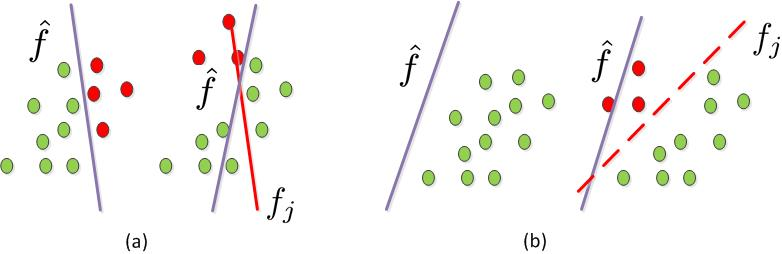
\includegraphics[scale = .6]{fig/domain.jpg}\\
  \caption{(a) Conventional adaptation method fail to find good initialization for the new category from source domain. (b) The parameters from $\hat{f}$ are more adaptive for the new categories.}
  \label{fig:wm}
\end{figure*}

\subsection{Experiment setup \& Evaluation}
We design the following experiment, transferring from Food-101 dataset to Food-220 dataset while just using a few examples to see the performance of our method. Since Food-101 has more images per category, we use it as the source domain. The fine-tuned GoogLeNet on Food-101 from Section \ref{sec:ft} is used as the feature extractor to generate feature representations for both datasets. Previous study suggests that deeper representations can achieve better performance \cite{hoffman2013one}, so deep feature representations from \emph{Pool5}, the layer before auxiliary linear classifier on top, are used as the inputs of our method.

%The types of food in Food-101 are mainly western style while most types of food in Food-220 are typical Asian foods. %They share about 36 categories even though the images in the same category may vary across these two datasets. These 36 duplicated categories are removed as noisy categories, so there are 220 new categories left in Food-256 dataset.
%To make this task more challenging, we also limited the number of examples in both source and target domain.

Baseline: To illustrate the advantage of our warm start strategy, we use the same model with random initialization (cold start) as the baseline.
Also, compared supervised adaptation techniques, such as A-SVM, from Table \ref{tab:su_domian} we can see that previous adaptation methods are not better than those model without adaptation.%The hypothesis of these adaptive methods limits their ability to adapt new categories as we discuss above.

\emph{5 shorts learning:} In our experiments, to build a balanced class distribution, the training set contains 5 randomly picked training examples from each category from both food datasets. To test the performance of our algorithm for new categories, the test set only contains all the rest examples in Food-220. For each step, we evaluate the accuracy of all adapted categories (learned categories in Food-220) among all learned categories.

For our SGD, we use effective learn rate following polynomial decay, to be 0 at max iteration and set base learning rate to 0.01 \cite{jia2014caffe}. We run SGD for 300 iterations for both warm start and cold start ensuring that they both converge.

%Unlike previous studies which consider the performance within the target domain separately, since the categories in our two datasets are in the general food category, we would rather considering to combine them together as a super-domain and evaluate the accuracy of target categories on this super-domain (In each step, the super-domain contains all the categories that have learned by our model).
\subsection{Adapting single new categories}
When there are multiple categories in target domain, our method divides the learning procedure into several steps and adapts one category in each step. The experiment starts with 505 training examples from Food-101 and in each step, we add 5 randomly picked examples from one category in Food-220 and train the new classifier as well as updating the other ones. So to adapt all the categories in Food-220 dataset, the algorithm starts from a 101 to 102 categories situation. We conduct the following experiment to test the first step of our method: we add an arbitrary new category from Food-220 to Food-101 and evaluate accuracy of the new category in the 102 learned categories. We run this experiment 220 times in each round, going through all the 220 categories. Table \ref{tab:N+1} shows the average performance of 10 rounds.

%\begin{table}[htbp]
%  \centering
%  \caption{Accuracy for a single new target category in M+1 experiment. Average top-5 accuracies for some categories are shown. Last row shows the average results for all categories.}
%    \begin{tabular}{c|cc|cc}
%    \toprule
%          & \multicolumn{2}{c|}{5 shots} & \multicolumn{2}{c}{1 shot} \\
%    \midrule
%       target category   & \multicolumn{1}{c}{Warm} & \multicolumn{1}{c|}{Cold} & \multicolumn{1}{c}{Warm} & \multicolumn{1}{c}{Cold} \\
%        \midrule
%    crape & \textbf{84.16} & 62.29 & \textbf{56.20}  & 28.00 \\
%   chip butty & \textbf{80.97} & 65.82 & \textbf{55.03} & 37.40 \\
%    meat loaf & \textbf{67.78} & 53.15 & \textbf{68.21} & 56.07 \\
%    dried fish & \textbf{92.00}    & 79.81 &\textbf{83.85} & 71.19 \\
%   scrambled egg & \textbf{75.21} & 63.54 & \textbf{59.00}    & 43.20 \\
%    pork belly & \textbf{81.76 }& 70.59 &\textbf{53.21} & 32.45 \\
%%    natto & 79.01&\textbf{80.70}&\textbf{73.69}&66.71\\
%%    miso soup &\textbf{96.06}&95.92&91.04&\textbf{94.52}\\
%    \midrule
%    %Average &\textbf{91.91$\pm$8.15}&88.82$\pm$10.40  & \textbf{80.77$\pm$ 12.03} & $71.78\pm 15.07 $ \\
%    Overall average &\textbf{91.91}&88.82  & \textbf{80.77} & 71.78 \\
%    \bottomrule
%    \end{tabular}%
%  \label{tab:N+1}%
%\end{table}%
\begin{table}[htbp]
  \centering
  \caption{Some results of top-5 Accuracy for adapting single new category.}
    \begin{tabular}{c|cc}
    \toprule
       new category   & \multicolumn{1}{c}{Warm} & \multicolumn{1}{c}{Cold}  \\
        \midrule
    crape & \textbf{84.16} & 62.29 \\
   chip butty & \textbf{80.97} & 65.82 \\
    meat loaf & \textbf{67.78} & 53.15 \\
    dried fish & \textbf{92.00}    & 79.81  \\
   scrambled egg & \textbf{75.21} & 63.54  \\
    pork belly & \textbf{81.76 }& 70.59  \\
    \midrule
    Overall average &\textbf{91.91}&88.82  \\
    \bottomrule
    \end{tabular}%
  \label{tab:N+1}%
\end{table}%

From Table \ref{tab:N+1} we can see that by taking advantage of the warm started parameters from negative classifier, the warm start classifiers does a slightly better than cold start ones in this experiment. Even though the difference of these two method is small after adapting just one category, we believe the margin of these two methods would increase as more new categories are learned.
%%%%%%%%%%%%%%%%%%%%%%%%%%%%%%%%%%%%%%%%%%%%%%%%%%%%%%%%%%%%%%%%%%%
\subsection{Adapting all new categories}
In this part, we show the performance of warm start in adapting multiple new categories situation. From the experiments above, warm start shows some improvement on cold start and in this part, we show that the improvement can be accumulated as more categories are learned and our method can outperform cold start with larger margin. In order to get consistent results, we have to add the new categories according to certain sequence in each step.
This sequence is determined by its original class index in Food-220. We run this experiment 10 times to eliminate the randomness caused by the training set and show the average results for both warm and cold start in Figure \ref{fig:wama} .

\begin{figure*}
  \centering
    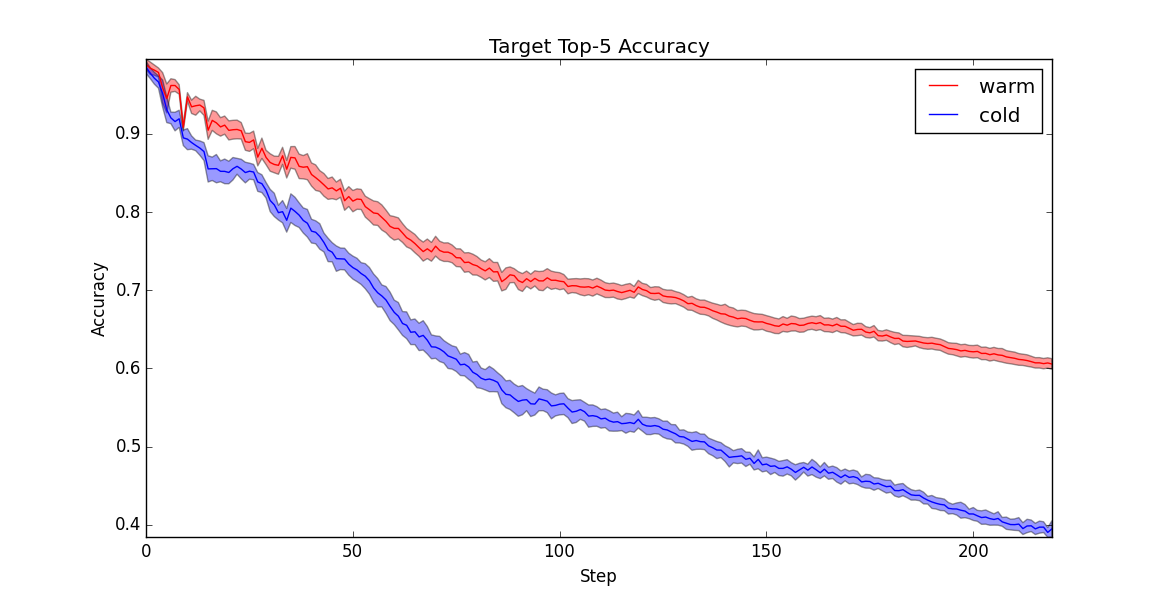
\includegraphics[scale=0.4]{fig/M+N.png}
    \caption{Top-5 accuracy curve for categories in Food-220 in super-domain with 5 shots. Mean and standard deviation are shown.}
      \label{fig:wama}
\end{figure*}

From Figure \ref{fig:wama} we can see that benefitting from warm start, classifiers can benefit from the "good" parameters of the previous step and thus the margin between warm and cold starts increases as more new categories are learned. 
Moreover, we find that in each step warm started classifier converges better than cold start. We select some steps and show their learning curve in Figure \ref{fig:errdiff}. From Figure \ref{fig:errdiff} we can see that by taking advantage of the parameters from negative classifier, warm started classifier converges much faster than cold start. 
We also compare performance of our method using different training iteration and show the results after adapting all new categories in Table \ref{tab:it}. From Table \ref{tab:it} we can see that even training with 10 iterations, warm started classifier can still reach competitive results. All these evidences indicate that warm start the parameters from the negative classifier can help the model to achieve better results with fewer training iteration.

%Indeed, cold start may not converge well for just 50 iterations. We believe that given enough training iteration, warm start can still converge to a better result (see Figure \ref{fig:errdiff}). We compare the results for different iterations and the average performance of 10 experiments are shown in Table \ref{tab:it}. The results of cold start in 10 and 20 iterations experiments, which are not even significantly better than random guess, are ignored. We observe that increasing training iteration won't help improve the performance of warm start very much as it converges very fast by taking advantage of better initialization.
\begin{figure*}[htbp]
\centering
\subfigure{
    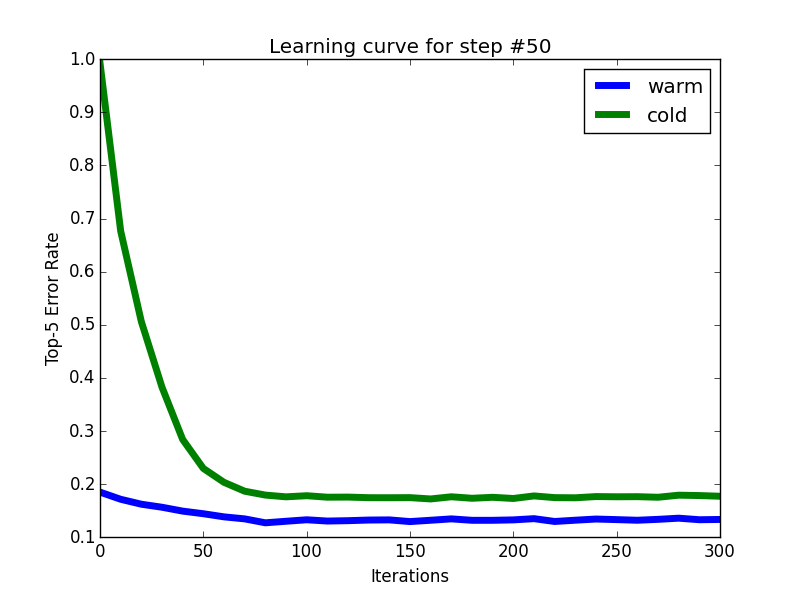
\includegraphics[width=0.3\textwidth]{fig/50W.png}
}
\subfigure{
    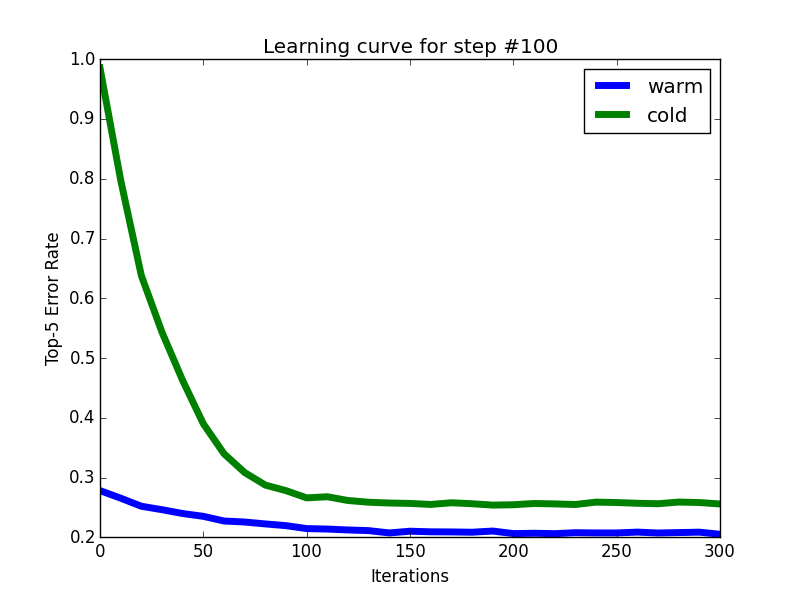
\includegraphics[width=0.3\textwidth]{fig/100W.png}
}\\
\subfigure{
    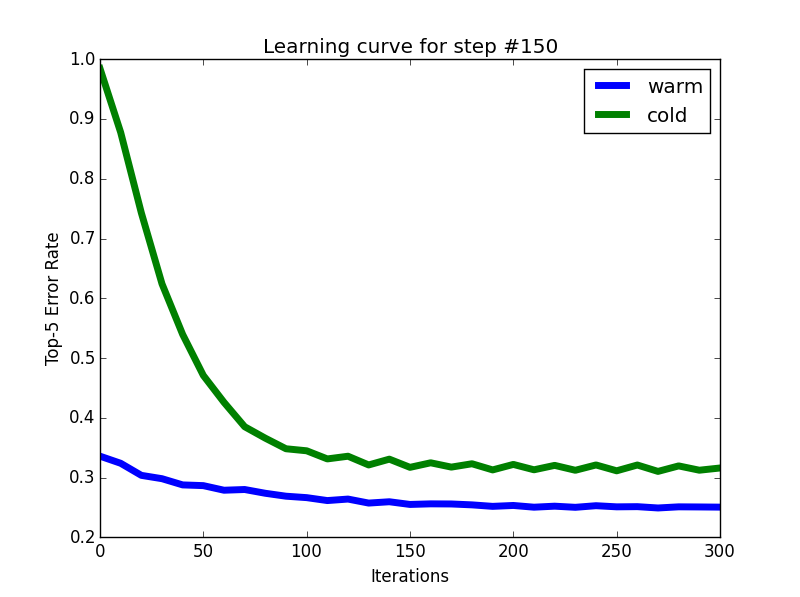
\includegraphics[width=0.3\textwidth]{fig/150W.png}
}
\subfigure{
    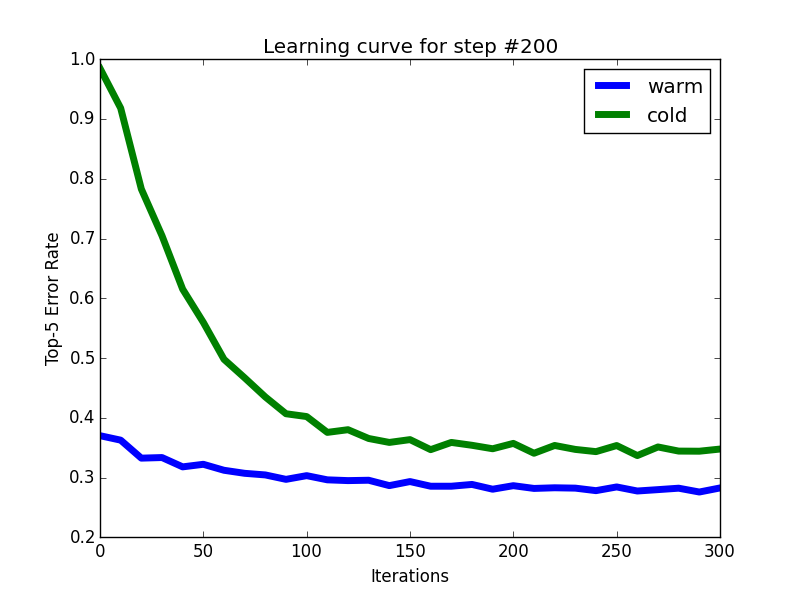
\includegraphics[width=0.3\textwidth]{fig/200W.png}
}
\caption{Overall learning curve in some steps for 300 iterations. \textbf{Observation:} even training with enough iteration, warm start can still outperform cold start in a single step.}
\label{fig:errdiff}
\end{figure*}
% Table generated by Excel2LaTeX from sheet 'Sheet1'
%\begin{table*}[htbp]
%  \centering
%  \caption{Overall top-5 accuracy for adapted categories in learned categories with different training iteration in each step.}
%    \begin{tabular}{C{1cm}cc|cc|cc|cc}
%    \toprule
%          & \multicolumn{2}{c|}{10 iterations}&\multicolumn{2}{c|}{20 iterations} &\multicolumn{2}{c|}{50 Iterations} & \multicolumn{2}{c}{300 iterations} \\
%    \midrule
%          & warm start& cold start  & warm start& cold start & warm start & cold start & warm start & cold start \\
%    Top-5& 60.37$\pm$ 0.58 & - &    60.54$\pm0.32$  &-&60.33$\pm$0.62   &     39.10$\pm$0.66   &    \textbf{61.48$\pm$0.59 }  & 55.35$\pm$0.48 \\
%    \bottomrule
%    \end{tabular}%
%  \label{tab:it}%
%\end{table*}%
\begin{table}[htbp]
  \centering
  \caption{Overall top-5 accuracy for adapted categories in learned categories with different training iteration in each step.}
    \begin{tabular}{C{1cm}c|c|c|c}
    \toprule
          & \multicolumn{1}{c|}{10 iterations}&\multicolumn{1}{c|}{20 iterations} &\multicolumn{1}{c|}{50 Iterations} & \multicolumn{1}{c}{300 iterations} \\
    \midrule
    Top-5& 60.37$\pm$ 0.58 &  60.54$\pm0.32$  &60.33$\pm$0.62&   \textbf{61.48$\pm$0.59 }   \\
    \bottomrule
    \end{tabular}%
  \label{tab:it}%
\end{table}%
